\title[Zahlensysteme]{Zahlensysteme und Kodierungen}

\subtitle{\emoji{woman-technologist} Mit Bits and Bytes rechnen}

\author[Blum, Cyril] % (optional)
{Cyril Blum \inst{1}}

\institute[KZN] % (optional)
{
  \inst{1}%
  Fachschaft Informatik\\
  Kantonsschule im Lee
}

\date[\today] % (optional)

\logo{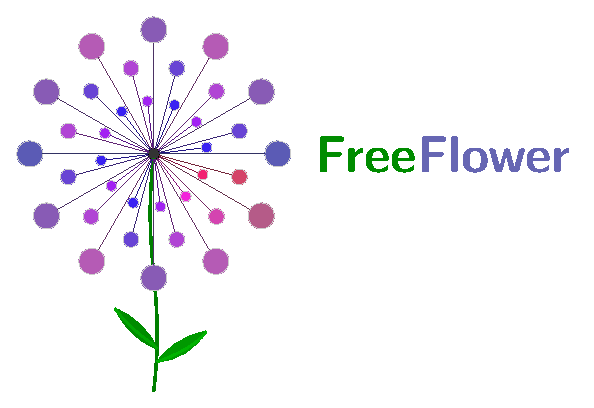
\includegraphics[width=2cm]{Logos/FreeFlower.pdf}}

\titlegraphic{\includegraphics[width=\textwidth]{"Grundlagen_Info/06_Datenbanken/Figures/title-emojis"}}

%The next statement creates the title page.
\frame{\titlepage}

\begin{frame}{Bits \& Bytes}
	\begin{itemize}[<+->]
		\item \textbf{bit} = \enquote{\textit{\underline{bi}nary digi\underline{t}}}, \enquote{binäre Ziffer} (eine 0 oder eine 1)
		\item \textbf{byte} = \enquote{Bissen} (von engl. \textit{\enquote{bite}}=Bissen aus 8 bits) \emoji{yum}
	\end{itemize}
\end{frame}


\begin{frame}{Bits \& Bytes}{Übersicht}
	\begin{enumerate}
		\item \faCheckSquare{} Zählen mit Bits
		\item \faSquare{} Rechnen mit Bits
		\item \faSquare{} Buchstaben codieren mit Bits
		\item \faSquare{} Farben repräsentieren mit Bits
	\end{enumerate}
\end{frame}



\begin{frame}[fragile]{Rechnen mit Zahlen}
	Addieren im Dezimalsystem ($49035_{10}$ + $718293_{10}$):
	\[
	\begin{array}{ccccccc}
	  & 0 & 4 & 9 & 0 & 3 & 5_{10} \\
	+ & \underset{}{7} & \underset{1}{1} & \underset{}{8} & \underset{1}{2} & \underset{}{9} & \underset{}{3_{10}} \\
	\hline
	 & 7 & 6 & 7 & 3 & 2 & 8_{10} \\\hline\hline
	\end{array}
	\]
	
\end{frame}

\begin{frame}[fragile]{Rechnen mit Zahlen}
	Nur 5 Regeln!
	\begin{itemize}
	\item 0 + 0 = 0 
	\item 0 + 1 = 1 
	\item 1 + 0 = 1 
	\item 1 + 1 = 0, Übertrag 1
	\item 1 + 1 + 1 = 1, Übertrag 1
	\end{itemize}
	
	Addieren im Binärsystem ($101011_2$ + $111010_2$):
	\[
	\begin{array}{ccccccc}
		& 1 & 0 & 1 & 0 & 1 & 1_2 \\
		+ & \underset{1}{1} & \underset{1}{1} & \underset{}{1} & \underset{1}{0} & \underset{}{1} & \underset{}{0_2} \\
		\hline
		1 & 1 & 0 & 0 & 1 & 0 & 1_2 \\\hline\hline
	\end{array}
	\]
\end{frame}

\begin{frame}{Auftrag}
Skript
\begin{itemize}
\item Zuerst Skript lesen \emoji{wink}
\item \aufgabebox{Aufgaben 1.11, 1.12, 1.14}
\item \aufgabebox{Aufgaben 2.1, 2.2}
\item \challengebox{Aufgabe 1.13}
\item \challengebox{Aufgabe 1.15}
\item \challengebox{Kurs auf Moodle (mit Tests)}
\end{itemize}
\end{frame}